\section{Estrutura}
A estrutura no ramo da engenharia é a área na qual utiliza de cálculos estruturais para dar forma a um objeto predefinido, determinando seus limites, materiais, estabilidade, dinâmica, vibração entre outros fatores. O objetivo da estrutura em um projeto é dar forma como um todo, levando em consideração cálculos estruturais analíticos ou mesmo simulações computacionais que facilitam na obtenção dos resultados. Além disso, com a parte estrutural pode-se integrar os demais subsistemas necessários.
Os principais fatores levados em consideração na análise estrutural de um projeto é se os materiais escolhidos são os melhores, mas com o melhor preço, se ele suportará as cargas aplicadas, não apresentando deformações plásticas e se o mesmo não sofrerá danos em decorrência de vibrações.

\subsection{Cálculos estruturais}

\subsubsection{Resistência dos materiais}

pós análise dos possíveis materiais a ser usado como reforço principal, escolheu-se o metalon de aço comum como primeira opção. Contudo, precisa-se verificar através de cálculos se o material resistirá aos esforços aplicados.


TENSÃO NORMAL:

O metalon tem como material principal o aço carbono simples, na qual é usinado com seção transversal quadrada e vazada. As suas propriedades são as seguintes:

\begin{itemize}
	\item Área transversal: 96mm²
	\item Tensão de escoamento: 350MPa
\end{itemize}

A massa que estará sobre a estrutura está estimada para ser em torno de 10kg. Assim, o peso sobre a estrutura considerando uma gravidade de 9,8m/s² será de 98N. Aplicando a fórmula seguinte tem-se a tensão aplicada na estrutura:

$\sigma$ = $\frac{F}{A}$

Onde F é a força aplicada e A é a área transversal da barra. Com isso, a tensão encontrada foi de 1,02MPa,  distribuindo para as quatro barras de apoio fica 0,26MPa, onde a tensão aplicada é de mais de 1000 vezes menor do que a barra suporta. 

FLEXÃO:

O material onde mais fica perceptível que ocorre flexão é a chapa de alumínio que servirá de fundo para a estufa. Assim, precisa-se calcular se não haverá ruptura. As propriedades do material são as seguintes:

\begin{itemize}
	\item Área transversal: 100mm²
	\item Tensão de escoamento: 241MPa
\end{itemize}

Em seguida calcula-se a tensão que sofrerá o alumínio considerando que o momento aplicado de acordo com a força é de 36,7N/m, o momento de inércia da área transversal é 6,46x$10^{-9} m^4$ e o c é $10^{-3}$m.

$\sigma$ = $\frac{Mc}{I}$

Onde M é o momento aplicado no material, c é a distância entre o ponto neutro e a máxima distância da seção transversal e I é o momento de inércia. Com isso tem-se que a tensão aplicada é de 5,69MPa, na qual é 40 vezes menor do que a tensão de escoamento do alumínio.

\subsubsection{Vibração natural}

Existem duas formas de se calcular a Frequência natural de um sistema, através de Métodos Matemáticos ou Métodos Experimentais. O método matemático consiste em cálculos analíticos ou modelos matemáticos computacionais (ex. Elementos Finitos), que são capazes de identificar as frequências naturais de uma estrutura. Fica evidente nesse caso, que a máquina não precisa ser construída para as frequências naturais serem identificadas, ou seja, se tratando de métodos matemáticos, apenas o projeto é suficiente para o cálculo das frequências naturais. Os métodos experimentais consistem em identificar as frequências naturais na própria peça física, ou seja, ela já deve estar construída. A ideia desse método é provocar uma vibração para que o sistema analisado entre em ressonância (frequência de operação = frequência natural). [5]

No caso do nosso projeto, foi realizado o método matemático onde a análise modal, considerando todas as cargas e forças que atuarão no sistema foram analisadas através de simulações no software ANSYS. Com isso, para a determinação da frequência natural de Vibração da estrutura.  Logo, calculamos a Tensão Equivalente de Von Misses, como mostrado na seção de Simulações.

Um estudo da zona elástica do material da estrutura, no nosso caso, o Metalon (Aço), nos mostra as frequências naturais onde este material é capaz de suportar as vibrações que estejam dentro da vibração natural do material. Os dados para o Aço são mostrados na figura 11.

\begin{figure}[H]
 	\centering
 	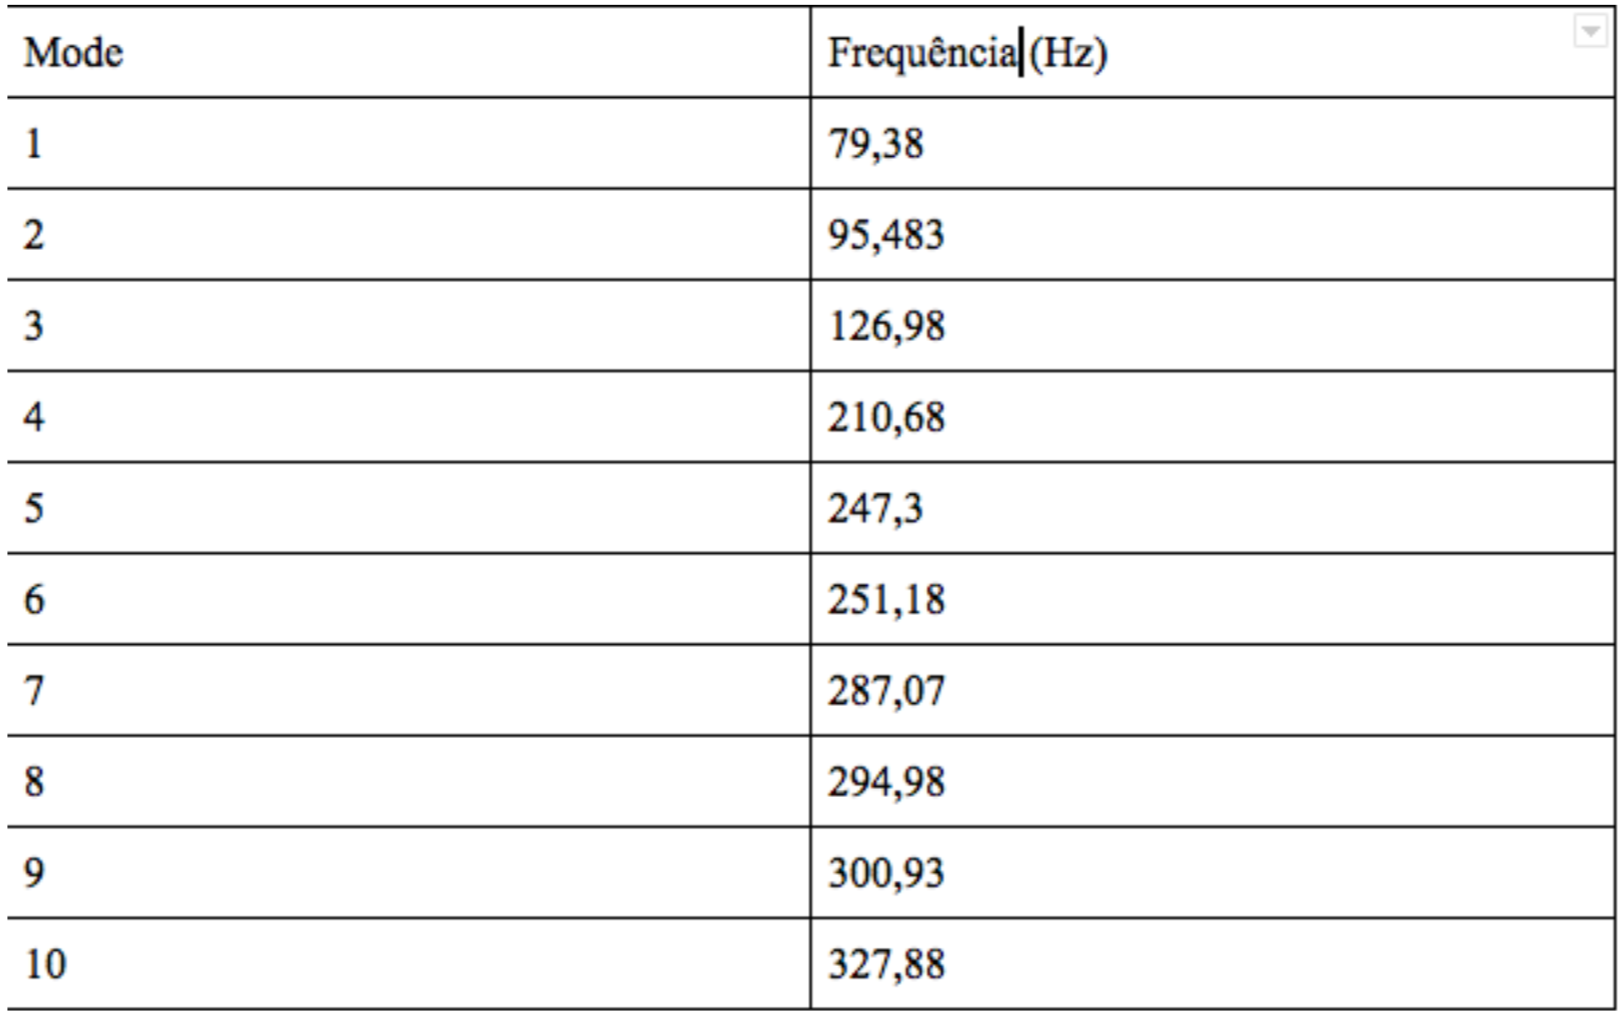
\includegraphics[width=10cm]{figuras/tabela_frequencia.png}
 	\caption{Tabela de Frequências Naturais  (Autoria Própria)} 
 	\label{tabela_frequencia}
\end{figure}

É importante ressaltar, que as mudanças realizadas na estrutura, através da utilização das chapas de MDF, Isopor e PVC, fazem com que a estrutura fique mais robusta, resistente e responde melhor as cargas com menores deformações. Analisando as tensões equivalentes de Von Misses com a tabela acima de vibração natural do Aço, podemos observar que após a análise estática foi feita a análise dos modos de vibração na estrutura, com as frequências naturais de vibração da estrutura é possível modificar as frequências de rotação dos motores instalados na estufa com o intuito de não excitar a estrutura, mantendo essas frequências bem longes e evitando com que ocorra o processo de Ressonância, podendo danificar a estrutura. [6]

\subsection{Simulações}

Como nem todos os componentes que farão parte final do projeto foram adquiridos, a equipe de estrutura não pode definir exatamente qual a massa que a estrutura suportará dentro de si. Desta maneira e tendo um tempo curto para a efetivação dos trabalhos, uma estimativa teve que ser feita. Após um brainstorm com integrantes de todas as áreas, a equipe chegou ao valor aproximado de 10kg, que engloba motores, sensores, válvulas, exaustores, plantário, tubos, canos, água, parafusos, roscas, reservatório e fiação.

Utilizou-se um fator de segurança 3 para qualquer tipo de inconveniente que possa ocorrer, ou seja, triplicamos a estimativa da massa esperada e encontramos o valor de 30kg. Arredondando o valor da aceleração da gravidade e utilizando a fórmula básica P=m.a encontramos uma força resultante axial sob a estrutura de 300 N. A equipe quis realizar diversos cenários de testes para checar o comportamento da estrutura mediante estes esforços e analisar as tensões de Von Mises e deslocamentos em diversas sessões do projeto a fim de buscar algum risco de ruptura. 

Como a massa estimada é muito baixa em relação ao que a estrutura pode suportar, as tensões e deslocamentos encontrados nas simulações conferem uma extrema segurança para o chassi levando em consideração os elevados limites de escoamento e ruptura que o material possuem, dando assim confiança e liberdade para que a equipe continue os trabalhos sem problemas.
Novas simulações serão feitas para o próximo ponto de controle, tendo em vista que haverá carga dinâmica que gerará momento fletor e uma melhor precisão sobre localização e presença dos componentes.

\subsubsection{CATIA}

\begin{figure}[H]
	\centering
	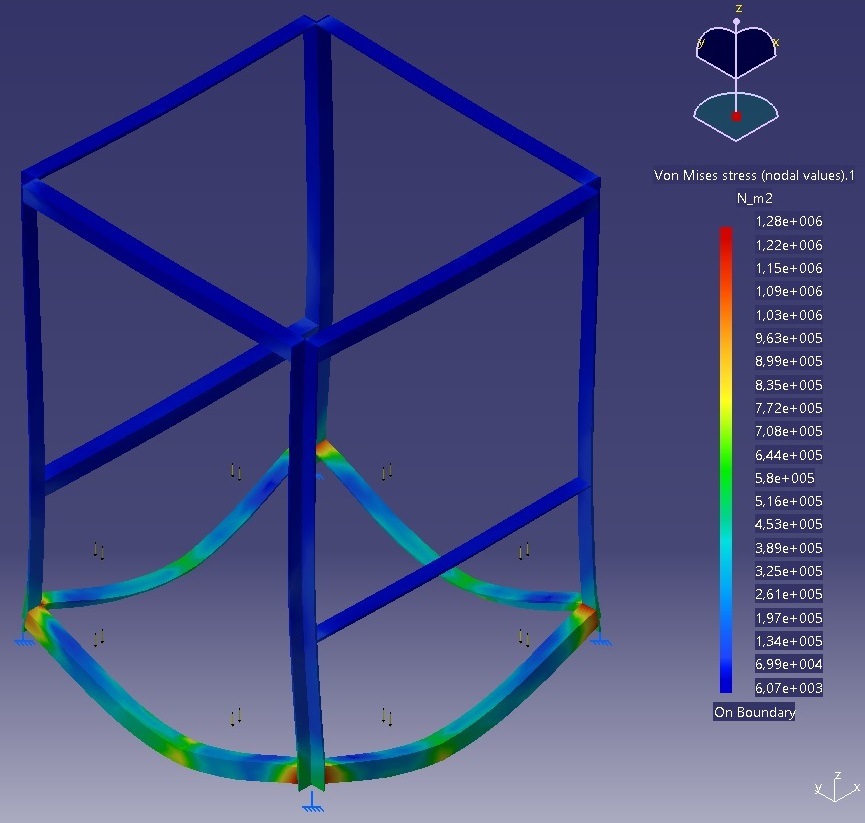
\includegraphics[width=10cm]{figuras/catia_1.jpg}
	\caption{Análise de Tensão Von Mises do chassi aplicando 300 N nas 4 faces do assoalho} 
	\label{catia_1}
\end{figure}

\begin{figure}[H]
	\centering
	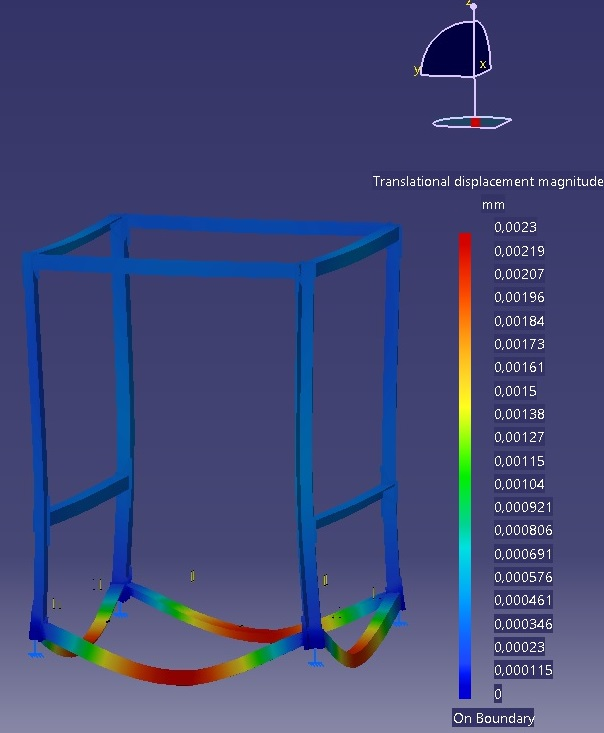
\includegraphics[width=9cm]{figuras/catia_2.jpg}
	\caption{Análise da magnitude da deformação do chassi aplicando 300 N nas 4 faces do assoalho} 
	\label{catia_2}
\end{figure}

\begin{figure}[H]
	\centering
	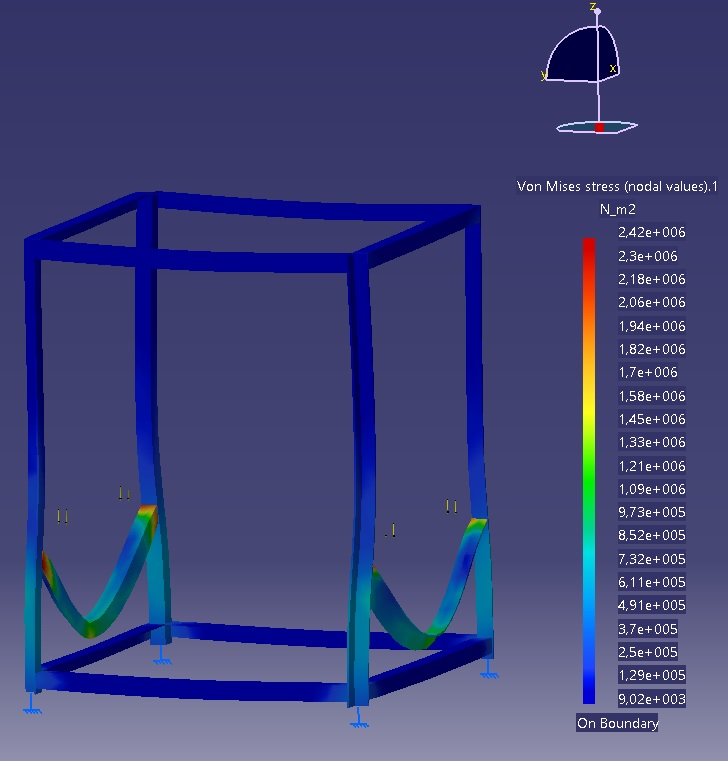
\includegraphics[width=9cm]{figuras/catia_3.jpg}
	\caption{Análise de Tensão Von Mises do chassi aplicando 300 N nas barras de suporte laterais} 
	\label{catia_3}
\end{figure}

\begin{figure}[H]
	\centering
	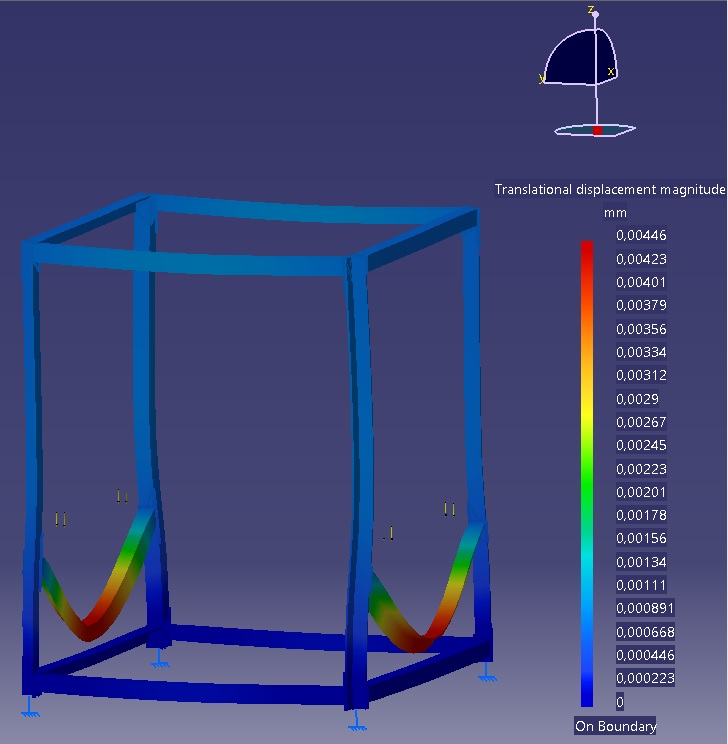
\includegraphics[width=9cm]{figuras/catia_4.jpg}
	\caption{Análise da magnitude da deformação do chassi aplicando 300 N nas barras de suporte laterais} 
	\label{catia_4}
\end{figure}

\begin{figure}[H]
	\centering
	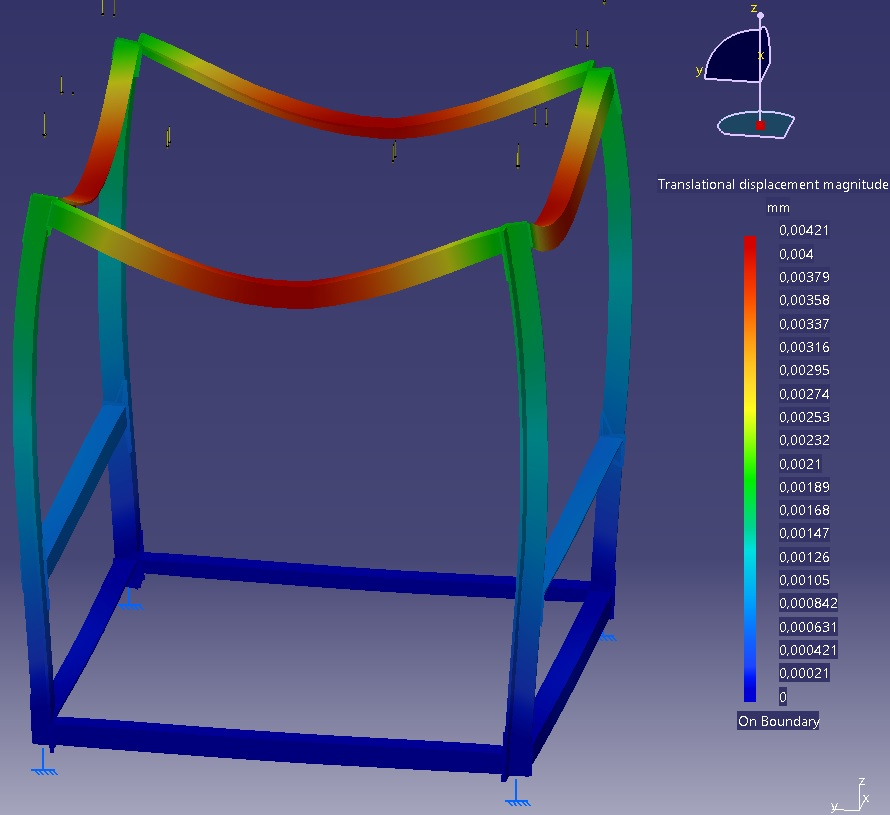
\includegraphics[width=9cm]{figuras/catia_5.jpg}
	\caption{Análise da magnitude da deformação do chassi aplicando 300N nas 4 barras do teto} 
	\label{catia_5}
\end{figure}

\begin{figure}[H]
	\centering
	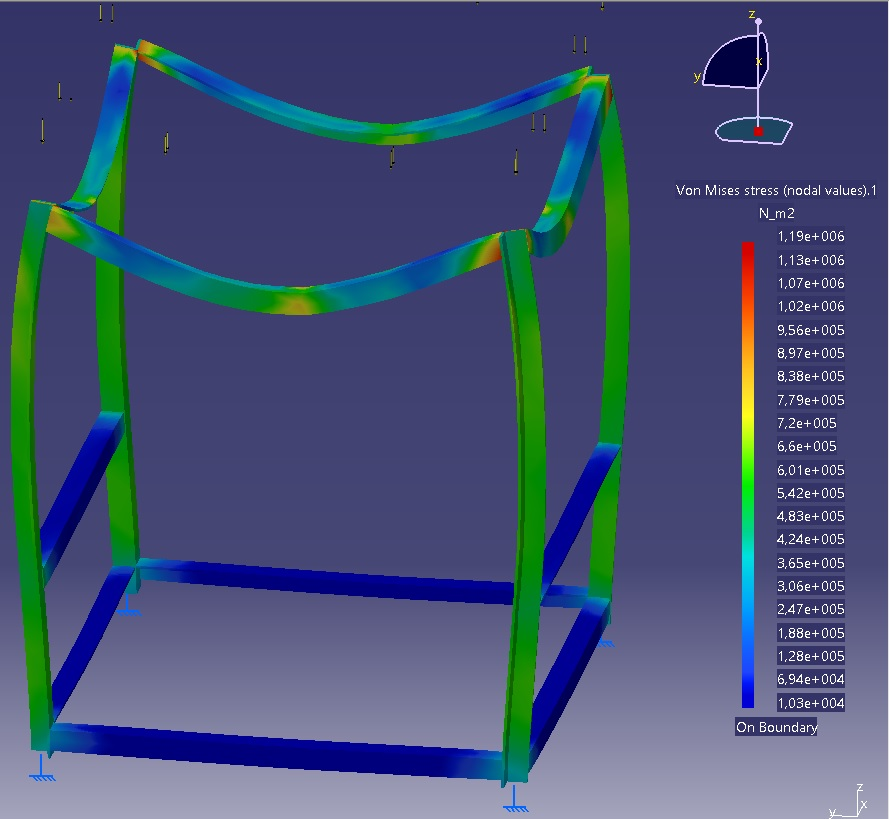
\includegraphics[width=9cm]{figuras/catia_6.jpg}
	\caption{Análise da tensão Von Mises no chassi aplicando 300N nas 4 barras do teto} 
	\label{catia_6}
\end{figure}

\begin{figure}[H]
	\centering
	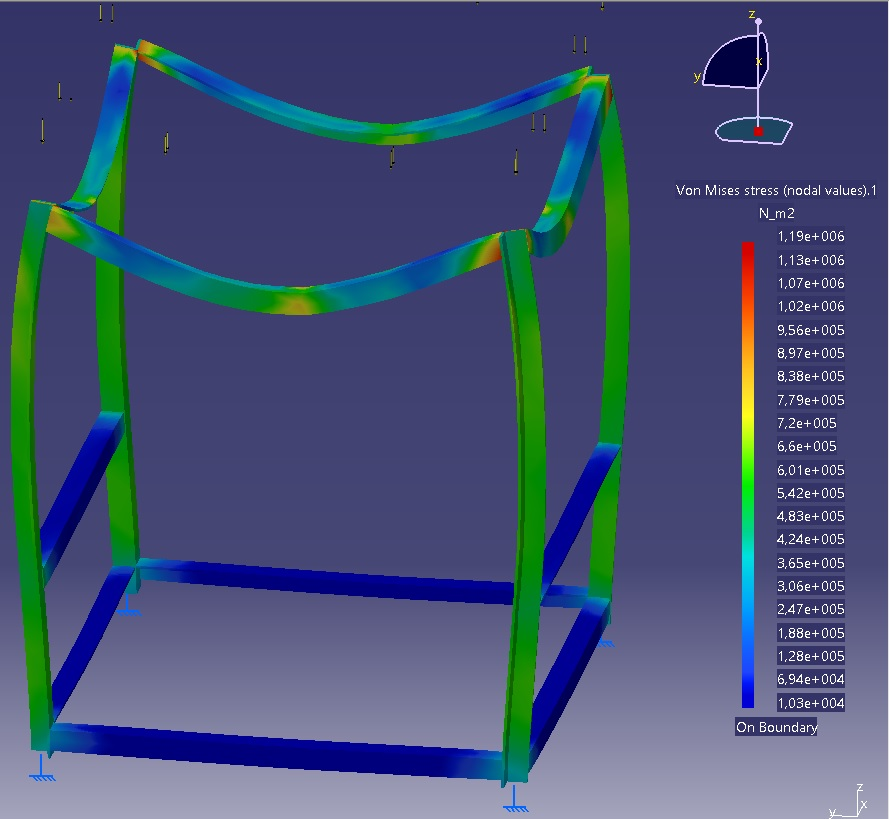
\includegraphics[width=9cm]{figuras/catia_7.jpg}
	\caption{Análise da tensão Von Mises no chassi aplicando 300N em todas suas faces do plano XY} 
	\label{catia_7}
\end{figure}

\begin{figure}[H]
	\centering
	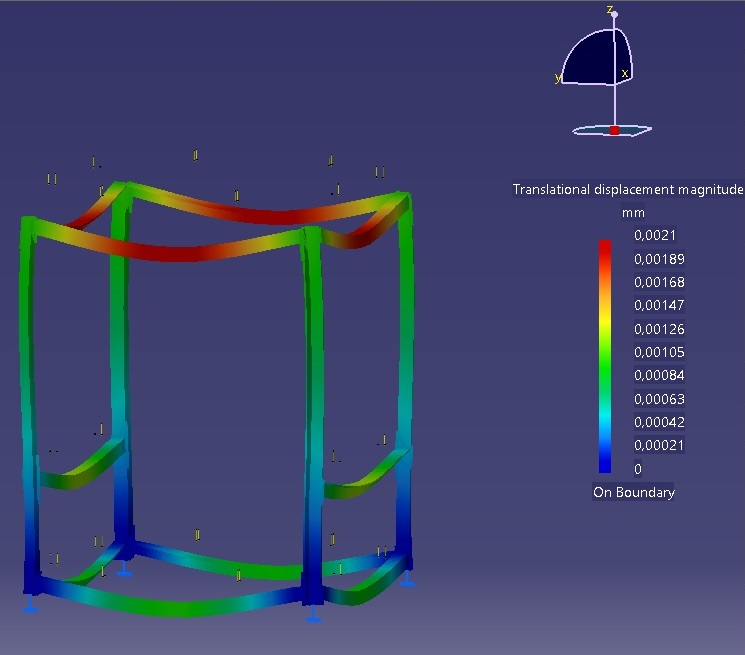
\includegraphics[width=9cm]{figuras/catia_8.jpg}
	\caption{Análise da da magnitude de deslocamento no chassi aplicando 300N em todas suas faces do plano XY} 
	\label{catia_8}
\end{figure}

\begin{figure}[H]
	\centering
	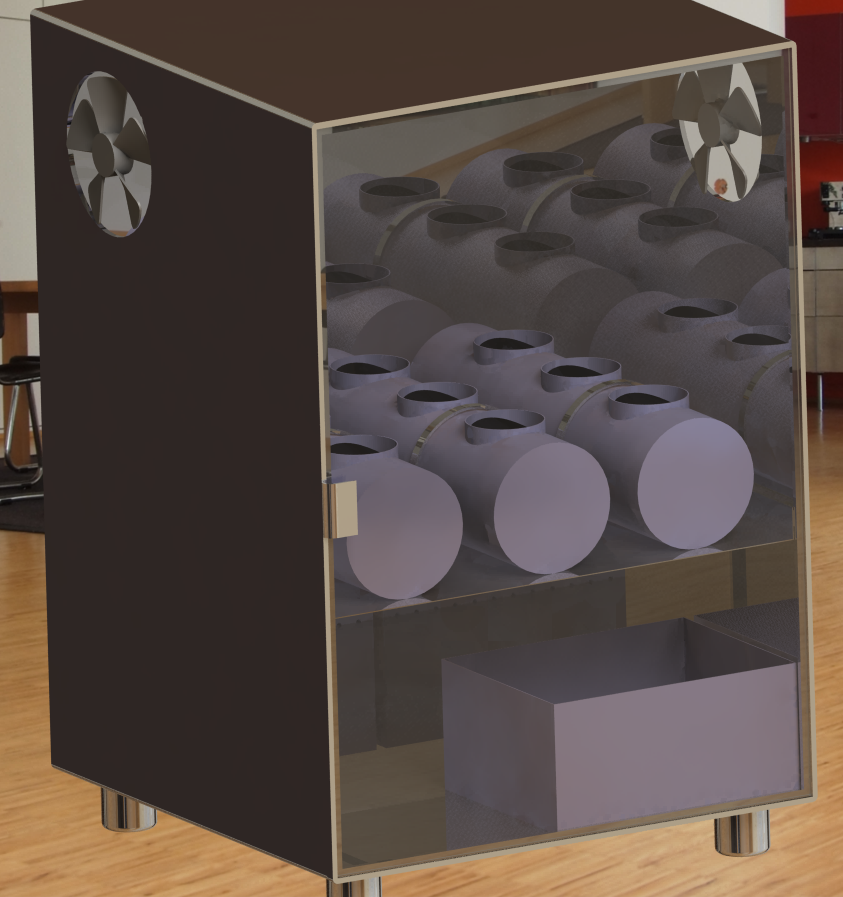
\includegraphics[width=9cm]{figuras/catia_9.png}
	\caption{Vista Frontal da Estufa Hidropônica simplificada} 
	\label{catia_9}
\end{figure}

\begin{figure}[H]
	\centering
	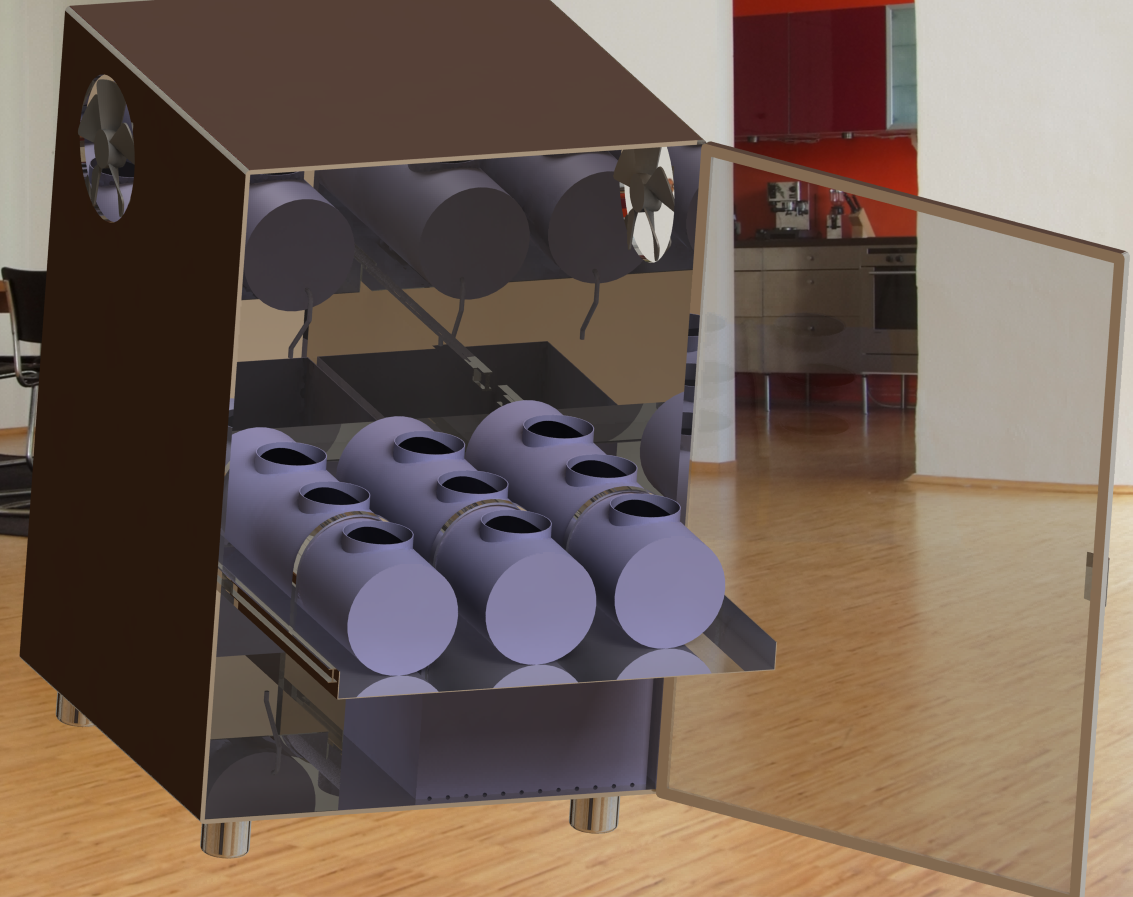
\includegraphics[width=9cm]{figuras/catia_10.png}
	\caption{Vista Frontal da Estufa Hidropônica simplificada com a porta aberta  e gaveta estendida} 
	\label{catia_10}
\end{figure}

\begin{figure}[H]
	\centering
	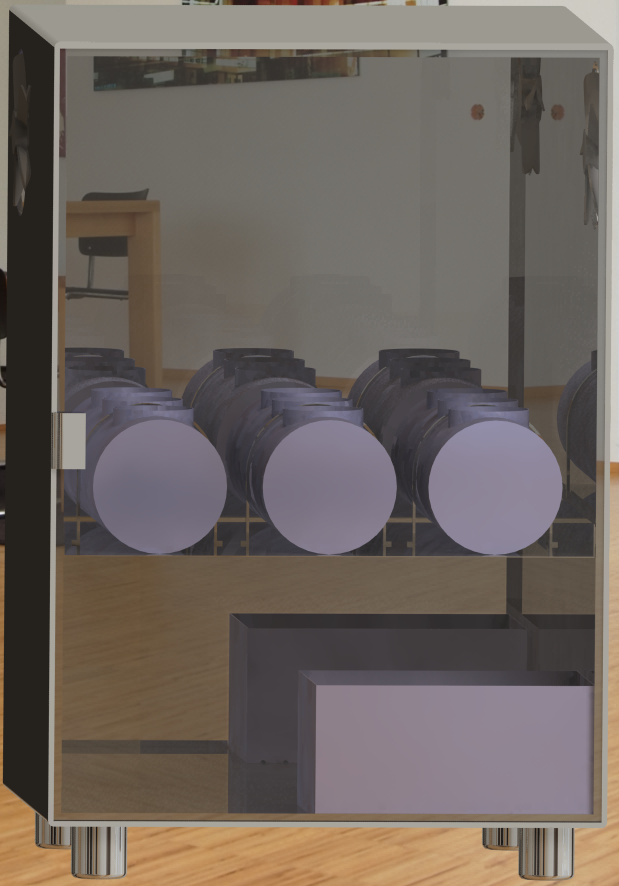
\includegraphics[width=9cm]{figuras/catia_11.png}
	\caption{Vista frontal da Estufa Hidropônica Simplificada com a porta fechada } 
	\label{catia_11}
\end{figure}
